\chapter{Referêncial Teórico}
\label{chap:referencial}
	
	Este capítulo é dedicado a uma exposição da fundamentação teórica de alguns elementos necessários à construção e funcionamento da bancada, bem como um estudo relacionado ao estado da arte.

	A fundamentação teórica é dividida em quatro seções, as quais descrevem sobre os projetos Mecânico, de Energia, Eletrônico e de Software respectivamente.

	\section{Revisão Bibliográfica: Mecânica}

	Nesta seção serão apresentados os componentes dos amortecedores, assim como os tipos de amortecedores que podem ser utilizados na bancada de testes e o sistema de excitação.

	\subsection{Componentes dos Amortecedores}
		Os amortecedores possuem diversos componentes, cada um com uma função específica. Os componentes do amortecedor serão especificados abaixo:

		\begin{itemize}
			\item \textbf{Corpo:}
		\end{itemize}

		Este possui uma câmera cilíndrica que tem como função principal conter o fluido do amortecedor, ou seja, o óleo utilizado, que gera a força do amortecedor. Na parte interna do cilindro é a região por onde o pistão deslizará, por isto é extremamente importante que esta contenha uma vedação para que o pistão desempenhe sua função corretamente. 


		O corpo também possui elementos de vedação e apoio da haste que permitirão o deslocamento da haste com o eixo axial sem que o fluido possa vazar para o exterior do cilindro. Esta parte do amortecedor também é responsável por receber as peças de montagem das molas e os pontos de fixação do amortecedor com a estrutura do veículo. 
		
		\begin{itemize}
			\item \textbf{Pistão:}
		\end{itemize}

			Esta parte do amortecedor divide o corpo em duas câmeras de óleo seladas, durante os movimentos de extensão e contração do amortecedor. Os orifícios do pistão são responsáveis pela comunicação entre estas duas câmeras. 


			O que determina o coeficiente de amortecimento é o tamanho desses orifícios e, por conseguinte a força que é gerada pela diferença de pressão entre as duas câmeras. 

		\begin{itemize}
			\item \textbf{Haste:}
		\end{itemize}

			A haste conecta o pistão com a estrutura do veículo, que por conseguinte transmite o movimento da massa não amortecida para o veículo. Esta parte também é encarregada de receber os elementos de fixação das molas, ou seja, tem que ser projetada de tal forma que resista as cargas de flambagem. 

		\begin{itemize}
			\item \textbf{Pistão flutuante:}
		\end{itemize}

			É o componente que tem a função de dividir o corpo do amortecedor, através de uma câmara de ar conhecida como reservatório de expansão, sendo necessário para acomodar o volume da haste que entra no corpo do amortecedor quando este sofre compressão.  De forma geral, quando o a haste se move em direção ao interior do corpo, faz com que o pistão fluente se movimente, com isto reduzindo o volume da câmara de ar, que por sua vez reduz o ar em seu interior. 


			A figura \ref{mecanica001} apresenta o esquema de um amortecedor com o pistão flutuante, separando a câmara de ar e óleo.

			\begin{figure}[h]
				\centering
				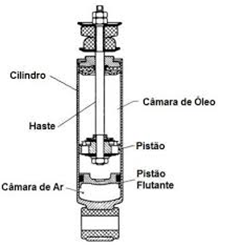
\includegraphics[scale=1]{mecanica001}
				\caption[Pistão Fluente separando câmara de ar e óleo]{Pistão Fluente separando câmara de ar e óleo \cite{DOliveira}}
				\label{mecanica001}
			\end{figure}

		\begin{itemize}
			\item \textbf{Válvula:}
		\end{itemize}

			As válvulas controlam o fluxo de óleo que passa pelo pistão, assim controlando a mudança do amortecimento de baixa velocidade para alta velocidade. A figura \ref{mecanica002} apresenta o trabalho das válvulas em compressão e extensão do amortecedor.

			\begin{figure}[h]
				\centering
				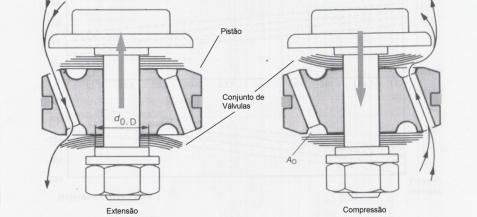
\includegraphics[scale=1]{mecanica002}
				\caption[Trabalho das válvulas durante a compressão e extensão do amortecedor]{Trabalho das válvulas durante a compressão e extensão do amortecedor \cite{DOliveira}}
				\label{mecanica002}
			\end{figure}

		\subsection{Tipos de Amortecedores}

			Independentemente do tipo de amortecedor, todos utilizam óleo para absorver a energia que a mola faz quando se passa por uma irregularidade na pista. Porem em condições extremas o óleo pode vir a criar bolhas, o que afeta de modo significativo o desempenho do amortecedor. Ao se utilizar o gás juntamente com o óleo este fica sobre pressão, assim diminuindo a possibilidade de o óleo borbulhar, ou seja, aumentando a performance do mesmo.


			De maneira geral o amortecedor a gás é melhor em termos dinâmicos quando comparado a um amortecedor a óleo. Porém os amortecedores pressurizados com gás se tornam mais elásticos, o que torna a suspensão do veículo mais rígida, assim tornando desconfortável o trajeto em pistas com irregularidades. 


			Para uma condução normal o máximo conforto é aconselhável para amortecedores a óleo, já para uma condução com maior ritmo é aconselhável amortecedores a gás, pelo fato de não entrarem em fadiga tão rápido quando coparados com os a óleo. As principais diferenças entre os amortecedores hidráulicos e a gás são mostradas na figura \ref{mecanica003}. 

			\begin{figure}[h]
				\centering
				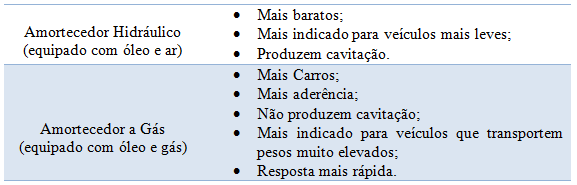
\includegraphics[scale=1]{mecanica003}
				\caption{Diferença entre os tipos de Amortecedores}
				\label{mecanica003}
			\end{figure}

			O projeto aqui proposto fará testes em amortecedores de veículos leves que segundo o código de Trânsito Brasileiro - CTB são veículos com até 3500Kg \cite{Portaria21}, para a maioria destes tipos de veículos são utilizados amortecedores a óleo. O funcionamento dos amortecedores a óleo será detalhado abaixo: 

		\subsubsection{Amortecedores Hidráulicos}
		
			O óleo é um lubrificante muito eficaz para diminuir o impacto do sistema de suspensão, este age nos tubos do pistão, onde existem válvulas que servem como passadouro do óleo. Esta atividade e a regulagem da válvula influenciam diretamente na resistência que o amortecedor fornece ao sistema. Este tipo de amortecedor é desenvolvido a todos os tipos de veículos do menor ao mais pesado, porem é mais indicado para veículos leves.

			Os amortecedores a hidráulicos podem ser subdivididos em dois tipos: os hidráulicos de dupla ação e os hidráulicos pressurizados.


			\begin{itemize}
			
				\item \textbf{Amortecedores Hidráulicos de Dupla Ação:} Este tipo de amortecedor é constituído por um conjunto de pistão e válvulas, onde estes componentes são fixados em uma haste que por sua vez se move em um tubo com óleo. As válvulas são os componentes necessários para a regulagem da passagem do óleo, assim controlando a velocidade da haste, o fluxo do óleo caracteriza a dupla ação do amortecedor.

				\item \textbf{Amortecedor Hidráulico Pressurizado:} Este amortecedor possui ar comprimido pressurizado em seu interior, que também é utilizado como fluido juntamente com o óleo. Ou seja, este amortecedor apresenta ambos os elementos, o óleo e o ar pressurizado. Porem este tipo de sistema está sujeito a perdas de pressão e falhas através da criação de bolhas de ar em seu interior.

			\end{itemize}

		\subsection{Princípio de Funcionamento dos Amortecedores}

			Amortecedores são dispositivos responsáveis pelo controle de oscilação das molas, nos veículos, através da conversão da energia cinética proveniente do movimento oscilatório das molas em energia termica. Existem diversos tipos de amortecedores utilizados por veículos, o amortecedor mais utilizado atualmente é o hidráulico mostrado na Figura \ref{amortecedor}, cujo princípio de funcionamento se dá basicamente pela passagem de óleo pelos furos do pistão, gerando o efeito amortecedor.

			\newpage
			\begin{figure}[!h]
				\centering
				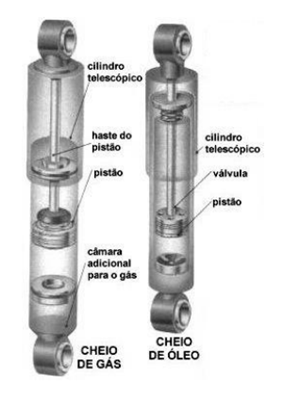
\includegraphics[scale=0.5]{amortecedor.png}
				\caption[Amortecedor Hidráulico]{Amortecedor Hidráulico \cite{Duarte}}
				\label{amortecedor}
			\end{figure}

			A dificuldade de passagem do óleo através dos furos do pistão, causada principalmente pelas características das anilhas (como diâmetro e espessura), as quais oferecem resistência à passagem do óleo, está diretamente relacionada ao efeito de amortecimento. Assim, quanto maior for a área livre de passagem para o óleo, definida muitas vezes pelas anilhas, menor será o amortecimento, visto que o escoamento se dá mais facilmente \cite{Duarte}.

			Os movimentos que os amortecedores permitem realizar são basicamente de extensão e compressão. Quando são realizados movimentos de extensão, como ilustra a Figura \ref{funcionamentoamortecedor} parte A, as válvulas de controle de tração são abertas e o óleo presente na câmara de tração é forçado para baixo, passando para a câmara de compressão. Sendo assim, a regulação da válvula de tração determina a medida de resistência que o amortecedor deverá fornecer ao sistema. Quando são realizados movimentos de compressão, como mostrado na Figura \ref{funcionamentoamortecedor} parte B, após a válvula do pistão ser aberta, o óleo é forçado para a câmara de tração e o controle das válvulas funciona analogamente ao de extensão \cite{Duarte}.

			\newpage
			\begin{figure}[!h]
				\centering
				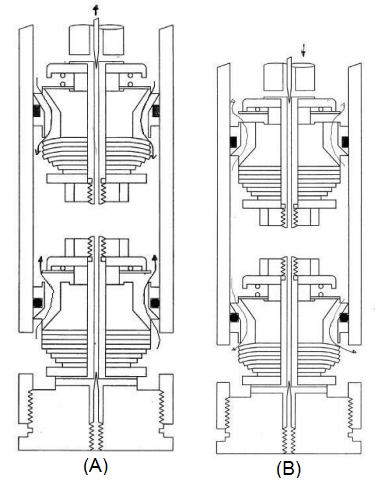
\includegraphics[scale=0.5]{funcionamentoamortecedor.png}
				\caption[Amortecedor durante o movimento de extensão(A) e de compressão (B)]{Amortecedor durante o movimento de extensão(A) e de compressão (B) \cite{Duarte}}
				\label{funcionamentoamortecedor}
			\end{figure}


		\subsection{Ensaios de Amortecedores}
			
			Em consideração à grande importância do controle de funcionamento de amortecedores, foram criadas, em meados da década de 90, as primeiras máquinas, conhecidas como Shock Dynamometer, capazes de testar o comportamento e tomar conhecimento das características próprias de cada amortecedor.
			O teste de amortecedores se faz importante principalmente por possibilitar a otimização do funcionamento dos amortecedores, assim como proporcionar, consequentemente, a melhora da estabilidade e segurança dos veículos, previnindo possíveis falhas  reduzindo riscos.
			Para se realizar ensaios de amortecedores existem opções de máquinas/sistemas que oferecem aplicações condizentes às solicitadas, para que seja simulada uma situação próxima à realidade, capazes de proporcionar a execução de testes de bancada para caracterização de um amortecedor. Neste trabalho, foram estudados quatro sistemas ,pinhão e cremalheira, elétropneumático, esteira com perfil de pista e o sistema biela manivela. Diante da análise de suas respectivas vantagens e desvantagens e de seus princípios de funcionamento, possibilitou-se a escolha de qual deles se adequaria melhor ao escopo do projeto. Entre os sistema estudados foi escolhido o sistema biela manivela, que será descrito seus elementos e funcionamento a seguir.


			\subsubsection{Sistema Biela Manivela}

				Os principais elementos desse sistema são o motor, o disco excêntrico, que funciona como manivela, um sistema de bielas e um cilindro que controla e orienta o movimento da biela. Quando aplicado ao ensaio de amortecedores, esse sistema pode ser adaptado, de modo a permitir vários cursos do amortecedor, permitindo que a biela seja fixada em pontos diferentes (com distâncias variáveis) do disco excêntrico.

				\begin{figure}[!h]
					\centering
					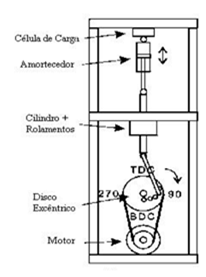
\includegraphics[scale=1]{sbm1.png}
					\caption[Ensaio de amortecedores por Sistema Bielo -Manivela]{Ensaio de amortecedores por Sistema Bielo -Manivela \cite{Dixion}} 
					\label{sbm1}
				\end{figure}

				A figura \ref{sbm2} mostra uma estrutura que suporta um motor elétrico ligado a um excêntrico por meio de uma correia, fazendo-o girar. A biela, por sua vez, está ligada a um veio, que está ligado no interior do cilindro, que está ligado a uma das extremidades do amortecedor.

				\begin{figure}[!h]
					\centering
					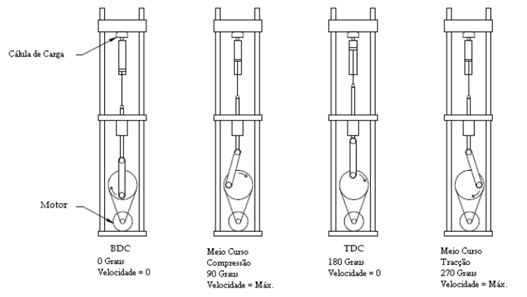
\includegraphics[scale=1]{sbm2.png}
					\caption[Funcionamento do Sistema Biela-Manivela]{Funcionamento do sistema biela-manivela \cite{Dixion}} 
					\label{sbm2}
				\end{figure}

%%%%%%%%%%%%%%%%%%%%%%%%% ENERGIA
	\newpage
	\section{Revisão Bibliográfica: Energia}

	Nesta seção serão apresentados os componentes necessários ao acionamento e ao controle de velocidade do sistema, bem como as formas de execução dos mesmos e do monitoramento de temperatura do amortecedor.

		\subsection{Motor de Indução Trifásico (MIT)}

			Motores elétricos têm por objetivo a transformação de energia elétrica em mecânica, sendo o motor de indução o mais utilizado devido a sua simplicidade de comando e seu baixo custo, comparado aos outros tipos de motores existentes \cite{Alexander}. Os motores elétricos se dividem em: motores de corrente contínua, que podem funcionar em amplos limites de velocidades, alta precisão e flexibilidade de controle, porém são motores de elevados custos, e motores de corrente alternada, que são mais utilizados devido ao fato da distribuição de energia elétrica ser feita normalmente em corrente alternada \cite{WEGMotorEletrico}.

			Os motores de corrente alternada são divididos em monofásicos, lineares e trifásicos. Os monofásicos são alternativas ideais para uso em locais onde não se dispõe de alimentação trifásica, pois são ligados a duas fases (tensão de linha) ou a uma fase e um neutro (tensão de fase). Os motores trifásicos são os mais utilizados nas indústrias, devido a sua longa vida útil e facilidade de operação \cite{WEGMotorEletrico}.

			Tanto os motores monofásicos quanto os trifásicos são divididos em máquinas síncronas e máquinas de indução. São chamadas de máquinas síncronas aquelas que, em condições de regime permanente, são máquinas de corrente alternada (CA) nas quais a velocidade é proporcional à frequência da corrente de sua armadura, assim o rotor gira na mesma velocidade que o campo magnético girante, resultando em um conjugado constante. Já as máquinas de indução, são aquelas onde o estator recebe diretamente a corrente alternada e o rotor recebe a corrente por indução a partir do estator, analogamente ao funcionamento de um transformador. Nesse caso, quando uma fonte polifásica equilibrada faz a excitação, produz-se um campo magnético no entreferro que gira na velocidade síncrona, a qual é determinada pelo número de polos do estator e pela frequência aplicada ao mesmo. O movimento relativo entre os enrolamentos do estator e do rotor produz a transformação de frequência, que é uma característica que diferencia o comportamento elétrico de uma máquina de indução ao de um transformador \cite{Fitzgerald}.

			O tipo de máquina de indução polifásica mais comumente usado é o rotor de gaiola de esquilo \ref{motorTrifasico}, no qual barras condutoras encaixadas em ranhuras no ferro do rotor e curto-circuitadas em cada lado por anéis condutores caracterizam seu enrolamento \cite{Fitzgerald}.

			\begin{figure}[!h]
				\centering
				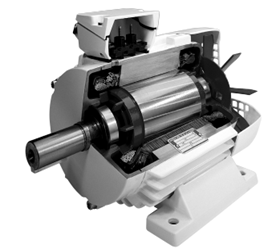
\includegraphics[scale=1]{motorTrifasico.png}
				\caption[Vista em corte longitudinal de um motor trifásico de gaiola de esquilo]{Vista em corte longitudinal de um motor trifásico de gaiola de esquilo \cite{Rockwell}} 
				\label{motorTrifasico}
			\end{figure}

			O funcionamento do MIT com acionamento direto pode ser explicitado pela curva abaixo, que relaciona torque x velocidade e escorregamento, mostrando que na partida de um motor ligado diretamente à rede o torque de partida será de aproximadamente 2 a 2,5 vezes o torque nominal. Além disso, a relação entre o escorregamento e a velocidade é inversamente proporcional, mostrando que o escorregamento varia diretamente com a variação de carga no sistema \cite{FitzgeraldETAL}.

			\begin{figure}[!h]
				\centering
				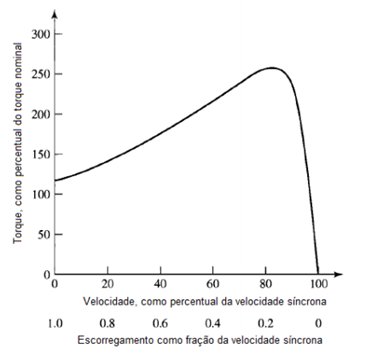
\includegraphics[scale=1]{curvaTorqueVelocidade.png}
				\caption[Curva Torque x Velocidade e Escorregamento para motores de indução trifásico]{Curva Torque x Velocidade e Escorregamento para motores de indução trifásico. Adaptado de \cite{FitzgeraldETAL}} 
				\label{curvaTorqueVelocidade}
			\end{figure}


		\subsection{Tipos de Partida para Motores de Indução Trifásicos}

			\subsubsection{Partida Direta}

				Nesse tipo de partida o motor é ligado diretamente à rede através de um contator, tendo como desvantagem o fato de sua corrente de partida ser de 5 a 6 vezes maior que a corrente nominal. Essa característica pode causar elevada queda de tensão no sistema de alimentação da rede e por isso os cabos devem ser superdimensionados, elevando consideravelmente os custos \cite{WEGMotorEletrico}. 


			\subsubsection{Partida Estrela-Triângulo}

				Baseia-se na redução de tensão nas bobinas durante a partida, podendo na ligação estrela, a corrente ser reduzida de 25\% a 33\% da corrente de partida na ligação triângulo \cite{WEGMotorEletrico}.  Para que seja possível esse tipo de partida é necessário que o motor possua seis ou mais terminais, tensão dupla, sendo necessário apenas possuir carga em seu acionamento após a rotação atingir 90\% da rotação nominal \cite{WEGMotorEletrico}\cite{Fitzgerald}. A vantagem desse método de acionamento do motor é a redução da corrente de partida em 1/3 em relação à partida direta e as desvantagens são a redução de 1/3 do torque nominal, a quantidade limitada de terminais e, caso a rotação do motor não atinja 90\% da velocidade nominal, o pico é equivalente ao de partida direta \cite{Alexander}.

			\subsubsection{Partida Eletrônica Soft-Starter}

				A partida eletrônica soft-starter funciona com uma tensão variável aplicada ao motor durante a aceleração. No final dessa partida, a tensão atinge um valor máximo pleno, após aceleração suave, formando uma rampa ascendente, onde a corrente de partida fica próxima à corrente nominal. A desvantagem associada à partida com soft-starter se dá pelo alto custo do equipamento \cite{WEGMotorEletrico}\cite{Fitzgerald}.


		\subsection{Controle de Velocidade de Motores de Indução}

			Motores de indução simples funcionam com velocidades relativamente constantes, porém existem várias aplicações que exigem diferentes velocidades ou uma faixa de velocidades ajustável continuamente \cite{WEGMotorEletrico}\cite{Fitzgerald}. Dessa forma, a velocidade síncrona de um motor de indução pode ser alterada por:

			\subsubsection{Variação do número de polos}

				Esse tipo de controle geralmente é aplicado a motores de polos ajustáveis, onde ocorre a mudança de números de polos na razão 2 para 1, sendo possível alterar qualquer das duas velocidades síncronas nas ligações da bobina. Nesse caso, o rotor do tipo gaiola de esquilo reage produzindo um campo de rotor que tem o mesmo número de polos do estator, tendo dois conjuntos independentes, podendo, desta maneira, variar até quatro velocidades síncronas distintas no motor\cite{WEGMotorEletrico}\cite{Fitzgerald}.

			\subsubsection{Variação da frequência de armadura}

				Baseia-se no controle de velocidade síncrona pela variação da frequência de armadura aplicada. A fim de se manter o fluxo constante, a tensão de armadura deve variar diretamente com a frequência (Volts/Hertz), conseguindo manter aproximadamente constante a indução magnética \cite{WEGMotorEletrico}\cite{Fitzgerald}.

			\subsubsection{Variação da tensão de linha}

				O torque interno desenvolvido por um motor de indução é proporcional ao quadrado da tensão de seus terminais primários. O baixo rendimento com escorregamento elevado é tolerado, porém existe a baixa capacidade de regulação de velocidade em relação a mudanças na carga \cite{WEGMotorEletrico}\cite{Fitzgerald}.

			\subsubsection{Variação da resistência do rotor}

				Método que utiliza características semelhantes ao controle de velocidade de motores CC em derivação através da resistência em série com a armadura. Suas principais desvantagens são o baixo rendimento quando a operação se dá em baixas velocidades e a margem limitada de regulação de velocidades \cite{WEGMotorEletrico}\cite{Fitzgerald}.

			\subsubsection{Variação do escorregamento}

				Baseia-se no controle de velocidade por dispositivos auxiliares, que permite a variação do escorregamento, respeitando as leis fundamentais de fluxo de potência em máquinas de indução \cite{WEGMotorEletrico}\cite{Fitzgerald}.


		\subsection{Inversor de Frequência}

			É um dispositivo eletrônico que transforma a tensão e a frequência da rede constantes em tensão e frequência variáveis. Ao variar a frequência da tensão de alimentação, varia-se o campo girante e, consequentemente, ocorre uma variação na velocidade mecânica de rotação do motor. A relação entre a frequência de alimentação, o escorregamento, o número de polos e a rotação de um motor é explicitada pela Equação abaixo:

			$$ n = \frac{120f}{p}*(1-s) $$

			Onde:
			\begin{itemize}
			\item $n$ = velocidade em rotação por minuto (rpm);
			\item $f$ = frequência da rede em Hertz (Hz);
			\item $s$ = escorregamento;
			\item $p$ = número de polos;
			\end{itemize}

			O inversor é composto por seis chaves que podem ser combinadas de forma a serem fechadas ou abertas e, com isso, pode se ter na saída do inversor, formas de ondas distintas \cite{WEGIF}.

			\begin{figure}[!h]
				\centering
				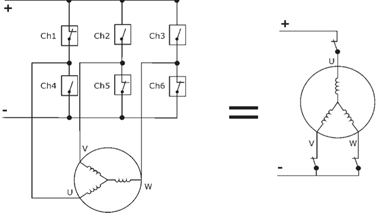
\includegraphics[scale=1]{confInversoFrequencia.png}
				\caption[Configuração do inversor de frequência chaveamento do sistema]{Configuração do inversor de frequência chaveamento do sistema \cite{WEGIF}} 
				\label{confInversoFrequencia}
			\end{figure}

			Nos acionamentos de motores utilizando dispositivos como o inversor de frequência, a curva de torque x velocidade apresenta, na maioria dos casos, outro comportamento, visto que agora o motor é acionado a diferentes frequências.

			\begin{figure}[!h]
				\centering
				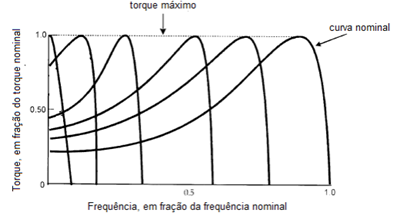
\includegraphics[scale=1]{curva2.png}
				\caption[Curvas de torque em diferentes frequências]{Curvas de torque em diferentes frequências \cite{Bose}} 
				\label{curva2}
			\end{figure}

		\subsection{Tipos de Controle do Inversor de Frequência}

			\subsubsection{Controle Escalar}

				Baseia-se na variação da tensão e da frequência (V/f) de forma a manter essa relação constante, assim como manter o torque do motor também constante e igual ao nominal, para diversas velocidades de funcionamento do motor \cite{WEGIF}. O controle escalar é o tipo de controle mais simples de ser implementado no inversor de frequência e é dividido em duas formas de variação de tensão por frequência: V/f e VVW, as quais se diferem pelo controle automático do escorregamento para VVW, pois haverá um cálculo para compensação de possíveis variações de carga e da rede elétrica, e pelo controle programável do V/f \cite{WEGIF}. Esses dois tipos de controle utilizam do mesmo conceito, porém a sua aplicação depende dos parâmetros que a carga exige, pois no controle V/F a velocidade e torque não são constantes, trabalhando em malha aberta, podendo variar a frequência com a relação de 1:20. Já no controle VVW, tem-se maior precisão para carga estática, com maior variação de velocidade de 1:30 e controle automático de possíveis ajustes que a carga necessita ou de variações da rede elétrica \cite{WEGIF}.

				O valor de indutância é uma constante do motor e a resistência é desprezada, porém a tensão e frequência são parâmetros que o inversor de frequência pode controlar \cite{WEGIF}. Assim o controle V/f constante, varia proporcionalmente com a variação da frequência de alimentação, conforme gráfico a seguir:

				\begin{figure}[!h]
					\centering
					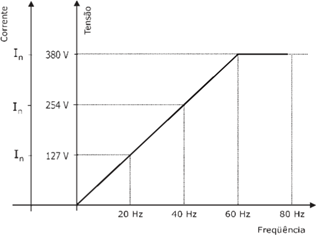
\includegraphics[scale=1]{graficoRT1.png}
					\caption[Comportamento do inversor de frequência]{Comportamento do inversor de frequência \cite{WEGIF}} 
					\label{graficoRT1}
				\end{figure}

				Para frequências abaixo de 30Hz, o termo de resistência não pode ser mais desprezado, pois influencia no cálculo da corrente. De modo que para baixas frequências, mantém-se a proporcionalidade entre frequência e a tensão, assim a corrente e o torque do motor diminuem consideravelmente \cite{WEGIF}. Para que esse fato seja evitado, aumenta-se a tensão do estator quando em baixas frequências, realizando o método denominado de compensação IxR, que compensa automaticamente por cálculos o valor de escorregamento que o motor possa sofrer, devido a variação de carga ou da rede, para baixas frequências \cite{WEGIF}.

				\begin{figure}[!h]
					\centering
					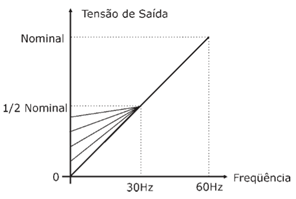
\includegraphics[scale=1]{graficoRT2.png}
					\caption[Comportamento da tensão na correção do escorregamento do MIT]{Comportamento da tensão na correção do escorregamento do MIT \cite{WEGIF}} 
					\label{graficoRT2}
				\end{figure}

				O método de controle escalar é geralmente utilizado para aplicações que não solicitam de grandes acelerações, frenagens, precisão e controle de torque. A sua precisão sem variação de carga é de até 0,5\% da rotação nominal, com variação de carga 3\% a 5\%, com torque de 0 a 100\% \cite{WEGIF}.

			\subsubsection{Controle Vetorial}

				No motor de indução a corrente do estator gera o fluxo de magnetização e o fluxo de torque, não aceitando obter um controle direto do torque. No controle V/f a referência de velocidade é usada como sinal para gerar os parâmetros tensão/frequência variável e disparar os transistores de potência. Já no controle vetorial a corrente necessária para produzir o torque requerido pela máquina é calculada através da corrente do estator e da corrente de magnetização \cite{WEGIF}.
				
				O controle vetorial utiliza de potentes transistores de potência para fazer cálculos em tempo real, para que sejam feitas as correções necessárias que a carga exige, por isso esse método é mais complexo, porém possui um grau de precisão maior. Esse tipo de controle divide-se em sensorless, vetorial com encoder, vetorial com encoder para motor PMSW e vetorial sensorless para motor PMSW. As duas últimas aplicações não serão citadas, pois fogem ao escopo do estudo de acionamento e controle do motor escolhido para atender a demanda que a carga necessita \cite{WEGIF}.
				
				O controle sensorless tem parâmetros que permitem alto torque e rapidez na resposta, para velocidade baixas ou na partida, não possui sensor de velocidade para o motor, sendo orientado pela corrente de campo, com variação de velocidade de 1:100. O controle vetorial com encoder, necessita do encoder no motor e interface para encoder no inversor, maior precisão, porém o custo de implementação tem custo alto \cite{WEGIF}.


		\subsection{Motor de Indução Utilizado como Gerador}

			Chamado de gerador de indução, o motor de indução opera como gerador quando é acionado por outra máquina, que faz com que o mesmo opere com uma rotação acima da síncrona e gere potência ativa que é entregue ao sistema no qual está conectado \cite{Medeiros05}. Esse tipo de máquina possui vantagens sobre o gerador síncrono, tais como menor custo e maior simplicidade. No entanto, o mesmo sofre alterações (decréscimos) de tensão conforme a carga aumenta, o que requer que o mesmo possua um sistema para controle da tensão. Isto ocorre devido a elevação da corrente da carga que provoca aumento na queda de tensão da máquina \cite{Medeiros05}.
			
			O controle de tensão geralmente é feio pelo uso de capacitores, que devem ser bem calculados, uma vez que o rendimento de um gerador de indução é diferente do rendimento do mesmo atuando como motor de indução. Isto pode ser um dos problemas durante a tentativa de realizar este tipo de ensaio. Outro fator que dificulta a correta aplicação das capacitâncias é que os capacitores podem apresentar uma diferença na capacitância nominal de 10\% para mais ou para menos. Os maiores problemas dessa aplicação são a alta corrente de partida e a regulação de frequência e tensão geradas durante o uso \cite{Monteiro}.
	 	
	 	\subsection{Freio de Prony}

			O freio de Prony é um método utilizado para aferir torque em eixos rotativos e também a potência mecânica da máquina, e foi proposto pelo engenheiro francês Gaspard Clair François Marie Riche de Prony em 1821. O dispositivo consiste em uma cinta resistente fixada em uma balança elástica em cada uma de suas extremidades, que considera as forças $F_{1}$ e $F_{2}$ aplicadas em cada uma das balanças \cite{Pereira}. 

			A força efetiva medida é o módulo da diferença entre os dois valores:

			$$ F_e= |F_1-F_2 | $$

			Com as forças medidas, pode-se então calcular o torque, como mostram a figura e equação a seguir, onde $F_{e}$ é o raio efetivo do rolamento e do eixo da máquina.

			\newpage
			\begin{figure}[!h]
				\centering
				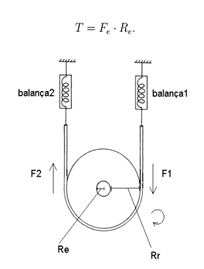
\includegraphics[scale=1]{torque.png}
				\caption[Medição de torque por freio de Prony]{Medição de torque por freio de Prony \cite{Calixto}} 
				\label{torque}
			\end{figure}

		\subsection{Monitoramento de Temperatura do Amortecedor}

			Os amortecedores comuns são geralmente compostos por um pistão dentro de um cilindro. O pistão possui pequenos furos que servem de passagem para o fluido (óleo existente dentro do amortecedor). Assim que o veículo encontrar um desnível no terreno, a mola entra em movimento, e o amortecedor deve acompanhá-lo, comprimindo e descomprimindo. No entanto, como o pistão possui pequenos orifícios, o fluido (óleo, gás) dentro do amortecedor passa em poucas quantidades elevando a pressão, o que faz com que o amortecedor reduza o movimento da mola, dissipando rapidamente a energia \cite{Dias}.
			
			O fluido mais comum utilizado nos amortecedores modernos é o óleo mineral fino, mas há diversas opções de óleos disponíveis no mercado que também podem ser utilizados em amortecedores e alguns amortecedores utilizam ar como fluido de amortecimento. O que diferencia os fluidos e suas aplicações são as suas propriedades. A massa específica e a viscosidade são as propriedades mais relevantes para a análise \cite{DOliveira}.
			
			Os amortecedores podem ser subdividos em muitas categorias, mas uma divisão mais geral pode ser dada classificando-os em hidráulicos e pressurizados. Entre as características  principais,  podemos  ressaltar  que  nos  amortecedores hidráulicos o óleo é forçado a passar de uma área de alta pressão para outra de baixa  pressão, como acontece nos percursos de compressão e de retorno. A súbita queda da pressão provoca a formação de bolhas no óleo. Chama-se este processo de cavitação e arejamento. Alguns amortecedores possuem maior quantidade de óleo no seu interior o que em certos casos é o mais indicado, pois demora mais para esquentar todo o conteúdo e assim suporta mais tempo resfriado para absorver os impactos provocados pelos terrenos irregulares, já que quanto mais aquecido o óleo, menos viscoso ele fica e, consequentemente, perde a ação, deixando a suspensão dependente apenas das molas \cite{Offshox}.
			
			A viscosidade absoluta, representada pela letra grega $\mu$ de um fluido é uma constante de proporcionalidade que relaciona a tensão de cisalhamento que o fluido sofre a uma determinada taxa de deformação, em um escoamento cisalhante puro:

			$$\tau_{xy} = \mu \frac{du}{dy}$$

			A viscosidade absoluta possui unidade de $Ns/m^{2}$ e seu papel é fundamental na performance do amortecedor, tendo em vista que influência diretamente no número de Reynolds que é utilizado para dimensionar o orifício do pistão \cite{Dias}.
			
			Um ponto importante que deve ser notado é que a viscosidade dos óleos minerais em geral varia amplamente em função da temperatura, com quedas de 2\% por cada aumento de 1 $^{\circ}C$. A figura a seguir ilustra esse fenômeno:

			\begin{figure}[!h]
				\centering
				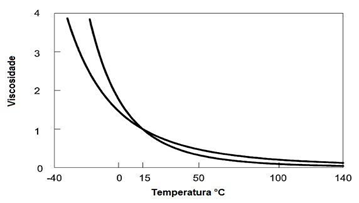
\includegraphics[scale=1]{graficoRT3.png}
				\caption[Variação da viscosidade de óleos minerais em função da temperatura]{Variação da viscosidade de óleos minerais em função da temperatura \cite{DOliveira}} 
				\label{graficoRT3}
			\end{figure}

			Esse efeito da temperatura sobre a viscosidade é indesejável, pois torna a performance do amortecedor variável e deve-se escolher o fluido de forma a reduzir esse efeito.
			
			As bolhas de ar, ao contrário do óleo, são compressíveis. Como tal, o movimento inicial do pistão de cada percurso comprime as bolhas antes que o óleo seja forçado a passar pela válvula.  Isto produz uma defasagem no controle do amortecimento, um problema que resulta consideravelmente a diminuição da eficácia do amortecedor. Já os amortecedores pressurizados contêm, o ar é substituído por gás, normalmente nitrogênio (gás inerte). A câmara com gás serve para comprimir o óleo evitando a formação de bolhas de ar, as quais nos amortecedores convencionais promovem a cavitação do pistão e geram instabilidade no sistema. Ou seja, a adição de gás sob pressão limita o efeito da formação de espuma de forma a conceder ao amortecedor uma maior eficácia e tempo de resposta muito mais preciso e imediato \cite{Pereira}.
			
			Durante o ensaio de um amortecedor na bancada de testes, faz-se necessário estudar a influência de algumas variáveis, sendo a temperatura, uma das mais importantes na análise do comportamento do amortecedor. Com estes estudos podem-se obter conclusões sobre as aplicações dos amortecedores em estudo. O amortecedor possui diversos componentes que tem suas características variáveis com a temperatura, sendo alguns deles a borracha de vedação, o fluido amortecedor, o material da carcaça (caso seja viscoelástico), entre outros \cite{Aseka}.

			O objetivo neste quesito é analisar o comportamento do fluido amortecedor com a variação da temperatura durante o ensaio do amortecedor. Para isto, durante o ensaio haverá a medição da temperatura na carcaça do amortecedor por meio de um sensor de infravermelho.
		
			Como a temperatura da carcaça não é equivalente à temperatura do fluido, utilizou-se de um estudo de transferência de calor em escoamentos de fluidos para encontrar um gradiente de temperatura que calculasse a temperatura equivalente.
		
			O fluido presente no amortecedor GL12380 que será usado na bancada de teste é um óleo tipo ATF, que possui as seguintes propriedades:

			\begin{figure}[!h]
				\centering
				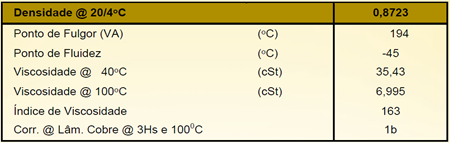
\includegraphics[scale=1]{propOleo.png}
				\caption[Propriedades do óleo tipo ATF]{Propriedades do óleo tipo ATF \cite{Petrobras}} 
				\label{propOleo}
			\end{figure}

			Com estudos utilizando os softwares MATLAB e ANSYS, pode-se chegar ao modelo matemático para realizar os cálculos da temperatura do fluido amortecedor e assim, atestar seu desempenho, já que a temperatura influencia diretamente na viscosidade do mesmo.


%%%%%%%%%%%%%%%%%%%%%%%%% ELETRONICA

	\newpage
	\section{Revisão Bibliográfica: Eletrônica}

	Nesta seção serão apresentados os conceitos importantes utilizados para o desenvolvimento do projeto eletrônico. 

		\subsection{Pulse Width Modulation - PWM}
			
			Em virtude da necessidade de controle da tensão e, consequente, da potência entregue a uma carga, desenvolveu-se na década de sessenta uma técnica denominada Pulse Width Modulation (PWM), ou Modulação por Largura de Pulso, que se tornou um mecanismo com uma infinidade de aplicações possíveis como, por exemplo, em circuitos que envolvem o controle de velocidade de motores, ou intensidade luminosa, controle de servo motores, entre outros.
			
			Nesse tipo de modulação, o ciclo ativo do sinal é modulado, ou seja a largura do pulso é modificada de acordo com a amplitude do sinal modulador. A modulação por largura de pulso utiliza-se do mecanismo de comparação entre dois sinais de tensão, um de baixa frequência e um de alta frequência, denominado sinal da portadora. 
			
			Conversores CC-CC em geral utilizam um sinal de tensão contínuo como sinal de referência e um sinal em formato dente de serra como portadora. Já nos conversores CC-CA o sinal de referência é senoidal e o sinal da portadora possui padrão triangular.

			Segundo o teorema de Nyquist a frequência da portadora deve ser no mínimo duas vezes maior que a frequência do sinal de referência, no entanto utiliza-se no mínimo uma frequência dez vezes maior em função da necessidade de resolução no processo de reprodução do sinal. A figura \ref{mecanismopwm} exemplifica o mecanismo para uma portadora em forma de onda triangular.

			\newpage
			\begin{figure}[!h]
				\centering
				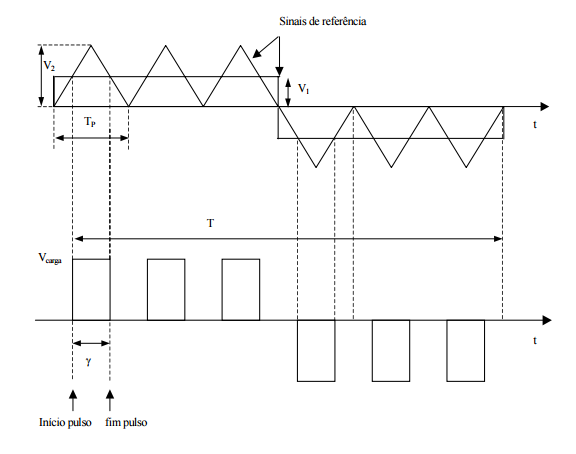
\includegraphics[scale=0.7]{mecanismopwm}
				\caption{Elementos Funcionais de um instrumento de medição}
				\label{mecanismopwm}
			\end{figure}

			O número de pulsos (N) depende da frequência da portadora para um período (T) do cilo pré-determinado, como pode ser visto na Figura \ref{mecanismopwm} é possível obter N por meio da seguinte equação:
													$$ N = \frac{T}{2T_p} $$
													
			A largura do pulso $\gamma$ varia em função das tensões V1 e V2 de referência, a equação que descreve tal relação é mostrada abaixo.

			$$ \gamma = \frac{\pi}{N}*\left(1 - \frac{V1}{V2}\right) $$


		\subsection{Características Básicas de Sensores}

			Segundo a definição de Thomazini, sensor é um dispositivo sensível a alguma forma de energia do ambiente para a qual é possível relacionar informações a cerca de alguma grandeza que precisa ser medida. O processo de escolha do sensor ideal para uma aplicação específica, assim como sua efetiva utilização, envolve diversos aspectos funcionais e operacionais. É fundamental, portanto, o conhecimento das principais características do sensor em questão tanto para processo de escolha, quanto para o processo de interpretação do datasheet e implementação do componente no sistema. De maneira geral, as características dos sensores podem ser divididas em características estáticas e características dinâmicas. Expõe-se a seguir alguns conceitos importantes inerentes ao processo de escolha do sensor em função do entrelaçamento das características dos mesmos com as peculiaridades do sistema.
				
			Características dinâmicas descrevem o comportamento do sensor em regime transiente, são tratadas matematicamente por equações diferencias e são amplamente influenciadas pelo ponto de operação. De acordo com a ordem do sensor é estruturado um modelo matemático capaz de representar o seu comportamento em regime transiente e em regime permanente, a partir da análise desse modelo é possível obter parâmetros importantes como o tempo de resposta. Tais características serão tratadas de acordo com os sensores escolhidos no processo de modelagem dos sensores.
				
			Características estáticas possuem uma variação desprezível com a utilização dos sensores, ou seja, referem-se a características que não sofrem mutabilidade com o tempo, como sensibilidade estática, histerese, limiar, faixa de operação,linearidade, espaço morto e resolução. 

			\subsubsection{Sensores de Proximidade}
				Em diversas áreas, industriais ou de algum segmento específico de consumo, a medição de distância é fundamental. Sensores de proximidade basicamente são sensores capazes de detectar a presença de algum objeto, assim como fornecer dados para mensurar a distância que o objeto se encontra. \\
				Deve-se selecionar o tipo de sensor a ser utilizado de acordo com o tipo de aplicação e, consequentemente, em função do seu mecanismo de operação. Essencialmente existem quatro mecanismos principais de medição de proximidade de um objeto: indutivo, capacitivo, ultrassônico e por infravermelho. Como sensores capacitivos e indutivos são utilizados em aplicações para baixa distância e alta resolução, eles não serão abordados nesse trabalho. 

			\subsubsubsection{Sensores de Infravermelho}
				Em geral esses sensores utilizam-se de técnicas de triangulação para calcular a distância de um objeto específico. Logo um pulso de luz infravermelha é emitido, que irá se propagar até encontrar um objeto, no encontro com o objeto a luz será refletida. Forma-se, portanto, um triângulo entre o emissor, o ponto de reflexão do objeto e o receptor. A Figura \ref{sensorinfra}  apresenta um comparativo em termos de faixa de operação de alguns modelos de sensores infravermelhos.
			
			\newpage
			\begin{figure}[!h]
				\centering
				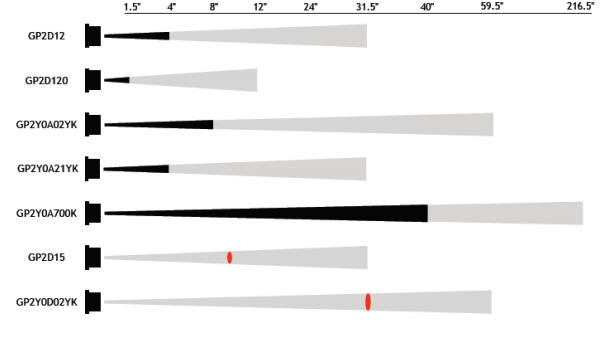
\includegraphics[scale=0.7]{comparativoinfra}
				\caption{Comparativo de Sensores Infravermelhos em termos de faixa de operação}
				\label{sensorinfra}
			\end{figure}

				Os traços em vermelho representam uma faixa de operação fixa, a região em preto o limiar e o extremo da região em cinza os máximos valores .


			\subsubsubsection{Sensores de Ultrassom}

			São sensores utilizados para medição de distâncias aplicando o princípio de propagação e reflexão sonora em um meio específico. A Figura \ref{diagramaultrassom} expõe um diagrama simplificado de um sensor de ultrassom:

			\begin{figure}[!h]
				\centering
				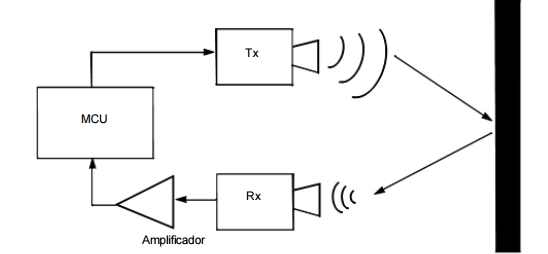
\includegraphics[scale=0.7]{diagramaultrassom}
				\caption{Diagrama funcional de um Sensor de Ultrassom}
				\label{diagramaultrassom}
			\end{figure}

				Dentro do espectro sonoro, ondas com frequências acimas de 20KHz são consideradas ultrassônicas, portanto esses sensores atuam na faixa de frequências correspondente à valores superiores a 20KHz. A velocidade de propagação está sujeita ao meio, no ar sabe-se que a velocidade do som, em condições normais de pressão, no nível do mar e em temperatura ambiente de $20\,^{\circ}\mathrm{C}$, é de aproximadamente 343 m/s. 
				
				Em termos de implementação, inicialmente deve-se enviar um sinal de trigger com uma duração específica para sinalizar o início do processo de medição, em seguida transmite-se um trem de pulsos com frequência de 40KHz através do módulo Tx. Caso o módulo Rx receba um sinal de retorno deve-se calcular a distância através da seguinte equação:
				$$ D = T(high)*V_{som}/2 $$
				
			\subsubsection{Sensores de Força}

				Células de carga são transdutores os quais tranformam a força, uma grandeza física, em um sinal elétrico. O funcionamento de uma célula de carga fundamenta-se no princípio de variação da resistência ôhmica de um extensômetro ao ser submetido à uma deformação. Alguns aspectos importantes devem ser considerados no processo de medição de força como  citado abaixo,
			\begin{itemize}

			\item Interferências – Temperatura, pressão e vibração atuam como fatores interferentes.
			\item Superfícies de carga – concentração de forças em uma parte específica do corpo de prova.
			\item Alinhamento do eixo -  pois força corresponde à uma grandeza vetorial, e a orientação é essencial.
			\item Estabilidade a longo prazo – relacionada aos processos de calibragem do sensor na posição zero.
			\item Fadiga do sensor – Relacionada ao ciclo de vida do sensor.
			\end{itemize}

				Existem diversos formatos de células de carga que devem ser escolhidos para uma aplicação específica em função de características como faixa de operação, limites dimensionais, resolução e custo. A Figura \ref{tiposcelula} e a Tabela \ref{tiposceluladecarga} apresentam diversos tipos de células de carga assim como suas respectivas faixas de operação.
				
			\begin{figure}[!h]
				\centering
				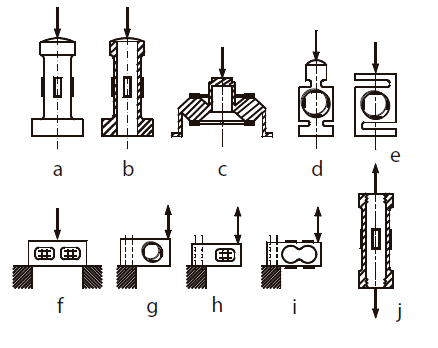
\includegraphics[scale=0.7]{tiposcelula.png}
				\caption{Tipos de Célula de Carga}
				\label{tiposcelula}
			\end{figure}

			\newpage
			\begin{table}[!h]
			\centering
			\caption{Cronograma de macros do projeto eletrônico}
			%\vspace{0.5cm}
			\begin{tabular}{ l l l }
			\hline
			\textbf{Identificador}	&	\textbf{Tipo} &	\textbf{\% Faixa de Operação}\\
			\hline
			a & Cilindro de compressão & 50kN - 50MN\\
			\hline
			b & Cilindro de compressão oco & 10kN - 50MN\\
			\hline
			c & Anel toroidal & 1kN - 5MN\\
			\hline
			d & Anel & 1kN - 1MN\\
			\hline
			e & Viga em S & 50N - 50kN\\
			\hline
			f & Feixe de flexão com dupla terminação & 20kN - 2MN\\
			\hline
			g & Feixe de flexão dupla (simplificado) & 500N - 50kN\\
			\hline
			h & Feixe de cisalhamento & 1kN - 500kN\\
			\hline
			i & Feixe de flexão dupla & 5N - 10kN\\
			\hline
			j & Cilindro de Tensão & 50kN - 50MN\\
			\hline
			\label{tiposceluladecarga}
			\end{tabular}
			\end{table}

%%%%%%%%%%%%%%%%%%%%%%%%% SOFTWARE

\newpage
\section{Revisão Bibliográfica: Software}

	Nesta seção será apresentada uma breve introdução ao Sistema Aprendizado de Máquina.

	\subsection{Sistema Aprendizado de Máquina}
			 
		O aprendizado de máquina é uma subarea de inteligência artificial, é apresentado por \cite{rezende_sistemas_2003} uma lista de paradigmas para aprendizado de máquina, a parti de suas características é possível classificar-los, sendo a linguagem de descrição, modo, paradigma e forma de aprendizado utilizado \cite{rezende_sistemas_2003}.

		Paradigmas para aprendizado de máquina\cite{rezende_sistemas_2003}:

		\begin{itemize}
		\item Simbólico
		\item Estatístico 
		\item Baseado em Exemplos
		\item Conexionista
		\item Genético
		\end{itemize}


		\cite{michalski_machine_1998} refere-se a divisão do aprendizado de duas formas, que podem ser classificados como caixa preta, onde não se fornece de forma fácil como o sistema chegou a aprendizado, e sistemas orientados ao conhecimento, aonde existes uma preocupação em explicar o como se chegou ao aprendizado.


		Redes neurais são do paradigma conexionista, elas são compostas por unidades mínimas chamado neurônio, cada neurônio pode ter diversas entradas, mas um única dado de saída, eles se tornam um nó em uma rede conectados por ligações direcionais, cada ligação tem seu peso para o neurônio\cite{russell_inteligencia_2013}.
			

		As formas como são montadas as conexões entre os neurônios define o tipo de rede neural, sendo elas, rede com alimentação para frente, tem conexões somente em um direção, rede de alimentação recorrente, elas usam retroalimentação, com isso a saída da rede volta para a entrada e é novamente processada, isso torna a rede mais complexa, podendo ter estados de estabilidade, oscilação ou caótico\cite{russell_inteligencia_2013}.

		Pretende-se desenvolver uma rede neural para a bancada, no entanto, ainda é necessário encontrar uma base de dados que possibilite o cruzamento de informações de amortecedores com os testes realizados na bancada. 


%%%%%%%%%%%%%%%%%%%%%%%%% FINAL
	\newpage
	\section{Estado da Arte}
	
		Uma das principais formas de testar um amortecedor é por meio de uma bancada de teste. Entre as razões para a realização desse tipo de teste estão: mensurar a performance, checar a durabilidade e testar modelos teóricos. Testes de amortecedores completos ou apenas de suas partes conferem validade para os modelos teóricos existentes. Já o teste de performance verifica se o amortecedor atende suas especificações com tolerância.  

		Os primeiros testes realizados em laboratório foram de vibrações livres transientes, em que utilizavam um bloco de concreto em uma mola de suspensão. Este teste com vibrações livres permitiu submeter o amortecedor a um ciclo realístico de uma operação transiente. Entre as principais vantagens deste tipo de teste estão: são fáceis de realizar, é um teste relativamente barato e não necessita de equipamentos capazes de gerar ciclos contínuos. Contudo, é um teste limitado, uma vez que, seus resultados não são tão bons comparados aos testes repetitivos de comportamento senoidal. 
	 
		Os testes cíclicos foram inicialmente realizados com a utilização de um mecanismo Biela-Manivela que por meio de um movimento alternado produzia uma onda senoidal. No entanto, a inclinação da haste desse mecanismo, introduz um movimento harmônico substancial ao movimento do amortecedor, o que descaracteriza a onda senoidal. Para solucionar esse problema, surgiu o mecanismo de Scotch Yoke que permite o alcance de uma onda senoidal perfeita. Testes eletromecânicos são apropriados para testes comparativos de baixa velocidade. Testes de grande porte utilizam mecanismo hidráulico. O teste hidráulico permite tanto teste de amortecedores quanto teste de uma suspensão completa. O mecanismo hidráulico também permite que testes transientes ou testes de ciclo único possam ser realizados. 
